\section{Ziel}
In diesem Versuch sollen das Emissionsspektrum einer Cu-Röntgenröhre und verschiedene Absoptionsspektren
aufgenommen und analysiert werden.

\section{Theorie}

\subsection{Erzeugung von Röntgenstrahlung}
Röntgenstrahlung kann durch beschleunigte Elektronen, die in ein Material eindringen, erzeugt werden. Dazu werden Elektronen aus einer Glühkathode emittiert und auf eine Anode hin beschleunigt.
Dies geschieht in einer evakuierten Röhre, da die Elektronen mit der Luft wechselwirken, wodurch dann keine Röntgenstrahlung erzeugt werden kann.
Die Röntgenstrahlung setzt sich aus dem kontinuierlichen Spektrum und der Bremsstrahlung zusammen, die im folgendem näher erleutert werden.

\subsubsection{Bremsstrahlung}
Fällt ein Elektron in ein Material ein, so kann dieses nah genug an einen Atomkern kommen, um von dessen elektrischen Feld beeinflusst zu werden. Durch die wirkende Coulombkraft wird dann das Elektron abgelenkt
und somit abgebremst. Dabei emittiert es einen Röntgenquant mit der Energie $\symup{\Delta} E$, die der verlorenden Energie des Elektrons entspricht.
Das Elektron kann durch die Coulombkraft auch so stark abgebremst werden, dass es seine gesamte kinetische Energie $E=U e_0$ abgibt, wobei $U$ der Beschleunigungsspannung und $e_0$ der Ladung des Elektrons entspricht.
Somit kann das Elektron beliebig viele Energieportionen abgeben, weshalb das Bremsspektrum kontinuierlich ist.
Ein schematischer Verlauf des Bremsspektrums ist in Abbildung \ref{fig:brems} zu sehen.
\begin{figure}
  \centering
  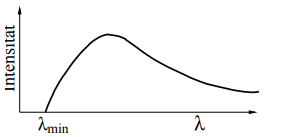
\includegraphics{Text/Bilder/Brems.png}
  \caption{Verlauf des Bremsspektrums \cite[1]{sample}}
  \label{fig:brems}
\end{figure}
Ein Röntgenquant verfügt über die minimale Wellenlänge $\lambda_\text{min}$, wenn das Elektron seine gesamte kinetische Energie abgegeben hat. Für sie lässt sich folgender Zusammenhang aufstellen:
\begin{equation}
  \lambda_\text{min}=\frac{h \cdot c}{e_0 \cdot U}
  \label{eqn:min}
\end{equation}

\subsubsection{Charakteristsches Spektrum}
Ionisiert ein Elektron das Materialso so, dass Leerstellen in einer inneren Schalen $n$ enstsehen, fällt ein Elektron aus einer höheren Schale $m$ in diese Leerstelle und emittiert dabei einen Röntgenquant.
Dieser verfügt dann über die Energie
\begin{equation}
  h \cdot \nu = E_m-E_n \text{,}
\end{equation}
weshalb das charakteristische Spektrum aus scharfen Linien besteht.
Diese werden mit $\xi_i$ bezeichnet. Dabei gibt $\xi$ an, auf welcher Schale (K, L, M..) der Übergang endet. Im Index werden für $i$ griechische Buchstaben ($\alpha$, $\beta$,..) verwendet.
Diese geben Auskunft über die Herkunft des Elektrons.
Die Feinstruktur der Linien, also dass jede Linie aus vielen, nahe beieinander liegenden Linien besteht, lässt sich damit erklären, dass die Elektronen aufgrund ihres Bahndrehimpulses und ihres
Elektronenspins unterschiedliche Energien besitzen.
Unter Berücksichtigung, dass Hüllenelektronen und die Wechselwirkungen zwischen den Elektronen generell das zu betrachtende Elektron vom Kern abschirmen,
kann die Energie eines Elektrons wie folgt beschrieben werden:
\begin{equation}
  E_N=-R_\infty z_\text{eff}^2 \cdot \frac{1}{N^2} \text{.}
\end{equation}
\begin{center}
 \tiny {($R_\infty=\SI{13.6}{\eV} \: \hat{=} \: \text{Rydbergenergie}$, $z_\text{eff}=z-\sigma$, $\sigma=\text{Abschirmungskonstante}$ )}
\end{center}

\subsection{Absorption}
Bei der Absorption von Röntgenstrahlung sind bei Energien von bis zu $\SI{1}{\MeV}$ der Photoeffekt und Comptoneffekt die dominierenden Prozesse.
%Bei zunehmender Energie nimmt der Absorptionskoeffizient ab.
Wie in Abbildung \ref{fig:abs} zu sehen ist, nimmt der Absorptionskoeffizient bei zunehmender Energie ab. \\
\begin{figure}[H]
  \centering
  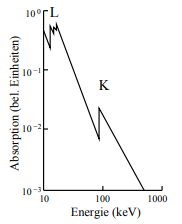
\includegraphics{Text/Bilder/absorbtion.png}
  \caption{Schematischer Verlauf des Energie-Absorptions-Graphen \cite[2]{sample}}
  \label{fig:abs}
\end{figure}
Die in Abbildung \ref{fig:abs} zu erkennende sprunghafte Steigung tritt immer dann auf, wenn die Photonenenergie gerade größer ist als die Bindungsenergie
eines Elektrons aus der nächsten inneren Schale. Dieser sprunghafte Anstieg wird auch als Absorptionskante bezeichnet. Im Vergleich mit der Absorptionsenergie
\begin{equation}
  h \nu_\text{abs}=E_n-E_\infty
\end{equation}
mit der Bindungsenergie eines Elektrons fällt auf, dass diese nahezu identisch sind. \newline
 Bei Betrachtung der Feintruktur können 3 L-Kanten ($L_\text{I}$, $L_\text{II}$, $L_\text{III}$)beobachtet werden.
Aufgrund der hier im Versuch verwendeten Technik, kann jedoch die $L_\text{I}$-Kante nicht von der $L_\text{II}$-Kante getrennt werden, wodurch nur 2 Kanten erkennbar sind.
Wird die Feinstruktur jedoch berücksichtigt, muss die Bindungsenergie eines Elektrons mit der Sommerfeldschen Feinstrukturformel beschrieben werden:
\begin{equation}
  E_\text{n, j}=-R_\text{\infty} \left(\frac{z_\text{eff, 1}^2}{n^2} +\frac{\alpha^2 z_\text{eff,2}^4}{n^3}  \left(\frac{1}{J+\frac{1}{2}}-\frac{3}{4n}\right)\right)
\end{equation}
\begin{center}
 \tiny {($\alpha=\text{Sommerfeldsche Feinstrukturkonstante}$, $J=\text{Gesamtdrehimpuls}$)}
\end{center}
Vereinfacht kann durch Bestimmung der Energiedeffierenz $\symup{\Delta} L$ zweier L-Kanten kann die Abschirmkonstante $\sigma_L$ bestimmt werden.
Für diese gilt:
\begin{equation}
  \sigma_L=Z-\left(\frac{4}{\alpha} \sqrt{ \frac {\symup{\Delta} E_L}{R_\infty} } -\frac{5\symup{\Delta} E_L}{R_\infty}\right)^{\frac{1}{2}} \left(1+\frac{19}{32}\alpha^2 \frac {\symup{\Delta} E_L}{R_\infty} \right)^{\frac{1}{2}}
  \label{eqn:sigL}
\end{equation}
\begin{center}
 \tiny {($\symup{\Delta} E_L=E_\text{II}- E_\text{III}$, $Z: \text{Ordnungszahl}$ )}
\end{center}
Bei bekannter Gitterkonstante kann die Energie $E$ auch mithilfe der Bragg-Refeltion experimentell bestimmt werden. Fällt Röntgenstrahlung auf ein dreidimensionales Gitter, so wird die Strahlung an den Atomen gebeugt.
Der Glanzwinkel $\theta$, bei dem konstruktive Interferenz auftritt, kann mithilfe der Bragg'schen Bedingung
\begin{equation}
  2d \sin{\theta} = n \lambda
\end{equation}
bestimmt werden.
